\chapter{Network}
\section{Proprietà dei grafi}
Quando le dimensioni dei grafi iniziano a crescere risulta difficile
rappresentarli in modo chiaro e comprensibile. Per questo motivo, quando si
lavora con grafi di grandi dimensioni, essi vengono rappresentati tramite
delle proprietà che ne descrivono la struttura.

Tra le proprietà più importanti troviamo:
\begin{itemize}
    \item \textbf{Lunghezza media dei cammini}: indica la lunghezza media dei
          cammini tra due nodi.
    \item \textbf{Diametro}: indica la lunghezza del cammino più lungo tra due
          nodi.
    \item \textbf{Grado di un nodo}: indica il numero di archi che partono o
          arrivano ad un nodo.
    \item \textbf{Coefficienti di clustering}: indicano la presenza di nodi
          vicini tra loro.
    \item \textbf{Centralità}: indica l'importanza di un nodo all'interno del
          grafo.
\end{itemize}
\subsection{Grado di un nodo}
\begin{definizione}[\textbf{Grado di un nodo}]
    Il \textbf{grado di un nodo} è il numero di archi che partono o arrivano ad
    un nodo. Nel caso di grafi diretti si parla di \textbf{grado uscente} o
    \textbf{out degree} e \textbf{grado entrante} o \textbf{in degree}.
\end{definizione}

Se si considera un grafo rappresentato attraverso una matrice di adiacenza, il
grado di un nodo può essere calcolato sommando i valori della riga o della
colonna corrispondente al nodo in questione. Nello specifico, se si considera
un grafo orientato, il grado uscente di un nodo corrisponde alla somma dei
valori della riga corrispondente al nodo, mentre il grado entrante corrisponde
alla somma dei valori della colonna corrispondente al nodo.

Più in generale possiamo riassumere il calcolo del grado di un nodo come segue:
\begin{equation}
    \text{Outdegree}(i) = \sum_{j=1}^{n} A_{ij} \quad \text{e} \quad
    \text{Indegree}(i) = \sum_{j=1}^{n} A_{ji}
\end{equation}
dove $A_{ij}$ è l'elemento della matrice di adiacenza corrispondente al nodo
$i$ e $j$. Nel caso di grafi non orientati, il grado di un nodo corrisponde
alla somma dei valori della riga o della colonna corrispondente al nodo in
questione.

Il grado di un nodo rappresenta una misura locale del grafo, nel caso in cui
si voglia ottenere una misura globale del grafo si può calcolare il grado
medio dei nodi. Tale misura può essere calcolata come segue:
\begin{equation}
    \langle k \rangle = \frac{1}{n} \sum_{i=1}^{n} \text{Grado}(i)
\end{equation}
dove $n$ rappresenta il numero di nodi del grafo. Anche in questo caso, se il
grafo è orientato dobbiamo distinguere tra grado uscente e grado entrante.
\begin{nota}
    Possiamo calcolare il grado medio anche come segue:
    \begin{itemize}
        \item Nel caso di grafi non orientati:
              \begin{equation}
                  \langle k \rangle = \frac{2E}{n}
              \end{equation}
              dove $E$ rappresenta il numero di archi del grafo.
        \item Nel caso di grafi orientati:
              \begin{equation}
                  \langle k \rangle = \frac{E}{n}
              \end{equation}
              dove $E$ rappresenta il numero di archi.
    \end{itemize}
\end{nota}
Una misura più rappresentativa della media dei gradi dei nodi è la \textbf{distribuzione
    dei gradi}. Possiamo definire $p(k)$ come la probabilità che un nodo abbia
grado $k$. Tale distribuzione può essere calcolata come segue:
\begin{equation}
    p(k) = \frac{n_k}{n}
\end{equation}
dove $n_k$ rappresenta il numero di nodi con grado $k$ e $n$ rappresenta il
numero totale di nodi del grafo. La distribuzione dei gradi può essere
rappresentata tramite un istogramma, in cui sull'asse delle ascisse vengono
inseriti i valori dei gradi, mentre sull'asse delle ordinate sono presenti i
valori di $p(k)$.
\begin{figure}[!ht]
    \centering
    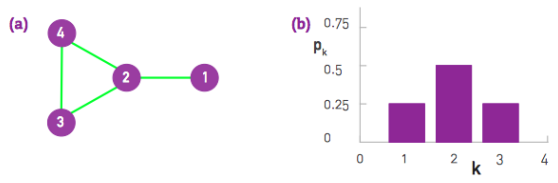
\includegraphics[width=0.7\textwidth]{./img/net/degreedist.png}
    \caption{Esempio di distribuzione dei gradi.}
    \label{fig:degree_distribution}
\end{figure}
\begin{nota}
    Questa distribuzione deve essere normalizzata, ovvero la somma di tutti i
    valori di $p(k)$ deve essere uguale a 1.
    \begin{equation*}
        \sum_{k=0}^{\infty} p(k) = 1
    \end{equation*}
\end{nota}

Il valore della distribuzione mi permette di rappresentare molti fenomeni dalla
robustezza della rete alla sua vulnerabilità.
\subsection{Cammino e distanza}
\begin{definizione}[\textbf{Cammino}]
    Un \textbf{cammino} è una sequenza di nodi in cui ciascun nodo è adiacente
    al successivo.
\end{definizione}
\begin{definizione}[\textbf{Distanza}]
    La \textbf{distanza} tra due nodi è definita come il numero minimo di archi
    che devono essere attraversati per andare da un nodo all'altro. Se i due
    nodi non sono collegati, la distanza è infinita.
\end{definizione}
Un modo semplice per calcolare la distanza tra due nodi è quello di utilizzare
l'algoritmo BFS (Breadth First Search).
\begin{definizione}[\textbf{Diametro}]
    Il diametro di un grafo è la distanza massima tra due nodi nel grafo.
\end{definizione}
\begin{definizione}[\textbf{Lunghezza media dei cammini}]
    La lunghezza media dei cammini è la media delle distanze tra tutti i nodi
    del grafo. Tale misura può essere calcolata come segue:
    \begin{equation}
        \langle d \rangle = \frac{1}{2E_{max}} \sum_{i \neq j} d_{ij}
    \end{equation}
\end{definizione}
Nei grafi non orientati, la lunghezza media dei cammini può essere calcolata
come segue:
\begin{equation}
    \langle d \rangle = \frac{1}{E_{max}} \sum_{i \neq j} d_{ij}
\end{equation}
dove $d_{ij}$ rappresenta la distanza tra i nodi $i$ e $j$ e $E_{max}$ rappresenta
il numero massimo di archi presenti nel grafo.
\subsection{Coefficienti di clustering}
\begin{definizione}[\textbf{Coefficienti di clustering}]
    I coefficienti di clustering sono una misura della presenza di nodi vicini
    tra loro. In particolare, il coefficiente di clustering di un nodo è una
    misura della probabilità che i vicini di un nodo siano collegati tra loro.
    Dato un nodo $i$ con grado $k_i$, il coefficiente di clustering locale è
    definito come segue:
    \begin{equation}
        C_i = \frac{2E_i}{k_i(k_i - 1)}
    \end{equation}
    dove $E_i$ rappresenta il numero di archi tra i vicini del nodo $i$.
\end{definizione}

Il valore di questo coefficiente può variare tra 0 e 1. Nel caso in cui il
coefficiente sia uguale a 1, significa che tutti i vicini del nodo $i$ sono
collegati tra loro. Nel caso in cui il coefficiente sia uguale a 0, significa
che nessun vicino del nodo $i$ è collegato ad un altro vicino.

Questa misura rappresenta la densità locale di un grafo. Per ottenere una
misura globale della densità del grafo, possiamo calcolare il \textbf{coefficiente
    di clustering medio}. Tale misura può essere calcolata come segue:
\begin{equation}
    \langle C \rangle = \frac{1}{n} \sum_{i=1}^{n} C_i
\end{equation}
dove $\langle C \rangle$ si può interpretare come la probabilità che due vicini
di un nodo, selezionato in modo casuale, siano collegati tra loro. 